
\tdi{Détailler les métriques définies
  figure \ref{fig:methode_rasterisation} + exemple}

\subsection{Classification}

Les \emph{métriques} que nous sommes amenés à construire peuvent être
de nature et porter sur ds phénomènes assez différents. Toutefois on
peut identifier une certaine récurrence dans leurs
caractéristiques.

Tout d'abord certaines \emph{métriques} quantifient des phénomènes
exprimés par rapport à \emph{l'objet de référence.}  C'est par exemple
le cas des matrices 4IM, utilisées précédemment pour introduire la
méthodologie de \emph{spatialisation.} En effet, la valeur de la
matrice calculée en un pixel dépend de la position et de la forme de
\emph{l'objet de référence,} si ce dernier change, la \emph{métrique}
sera caduque. Cependant des \emph{métriques} comme la pente ou
l'altitude, utilisées pour \emph{spatialiser} des \emph{indices de
  localisation} tels que : \enquote{Je suis à \SI{2500}{\meter}} ou
\enquote{Nous sommes dans une zone de forte pente}, ne dépendent pas
d'un \emph{objet de référence.} On parle dans ce cas de
\emph{métriques intrinsèques,} que l'on oppose aux \emph{métriques
  extrinsèques,} telles que la distance à \emph{l'objet de référence}
ou une relation topologique.

Un second critère peut être utilisé pour distinguer les
\emph{métriques.} En effet, certaines d'entre elles nécessitent un
paramétrage pour être calculées. 


\subsection{Métriques intrinsèques}

\tdi{Présentation des métriques qui ne dépendent pas de l'objet de
  référence -> elles sont calculables une fois. Ex : Pente, altitude
  absolue (mais déjà calculée vu que MNT).}

\tdi{Est-ce qu'on peut vraiment faire cette distinction ??}

\subsection{Métriques extrinsèques}

\tdi{Présentation des métriques locales, qui changent pour chaque
  \emph{objet de référence}, distance, orientation, visibilité}

\subsection{Métriques Paramétriques}

\subsection{Métriques non paramétriques}

\begin{table}
  \centering
  \begin{tabular}{>{\bfseries}R{3cm}C{5cm}C{5cm}}
  \toprule
  &
   \multicolumn{1}{c}{\bfseries Paramétriques} &
   \multicolumn{1}{c}{\bfseries Non Paramétriques} \\
  \midrule
  Extrinsèques &&Pente\\
  Intrinsèques &&\\
  \bottomrule
\end{tabular}

  \caption{Types de métriques}
  \label{fig:type_metriques}
\end{table}


\begin{figure}
  \centering
  \begin{tikzpicture}
  \tikzset{et/.style={above,font=\footnotesize\vphantom{Ag}}}
  %
  \node[inner sep=0pt, anchor=south west] (image) at (0,0){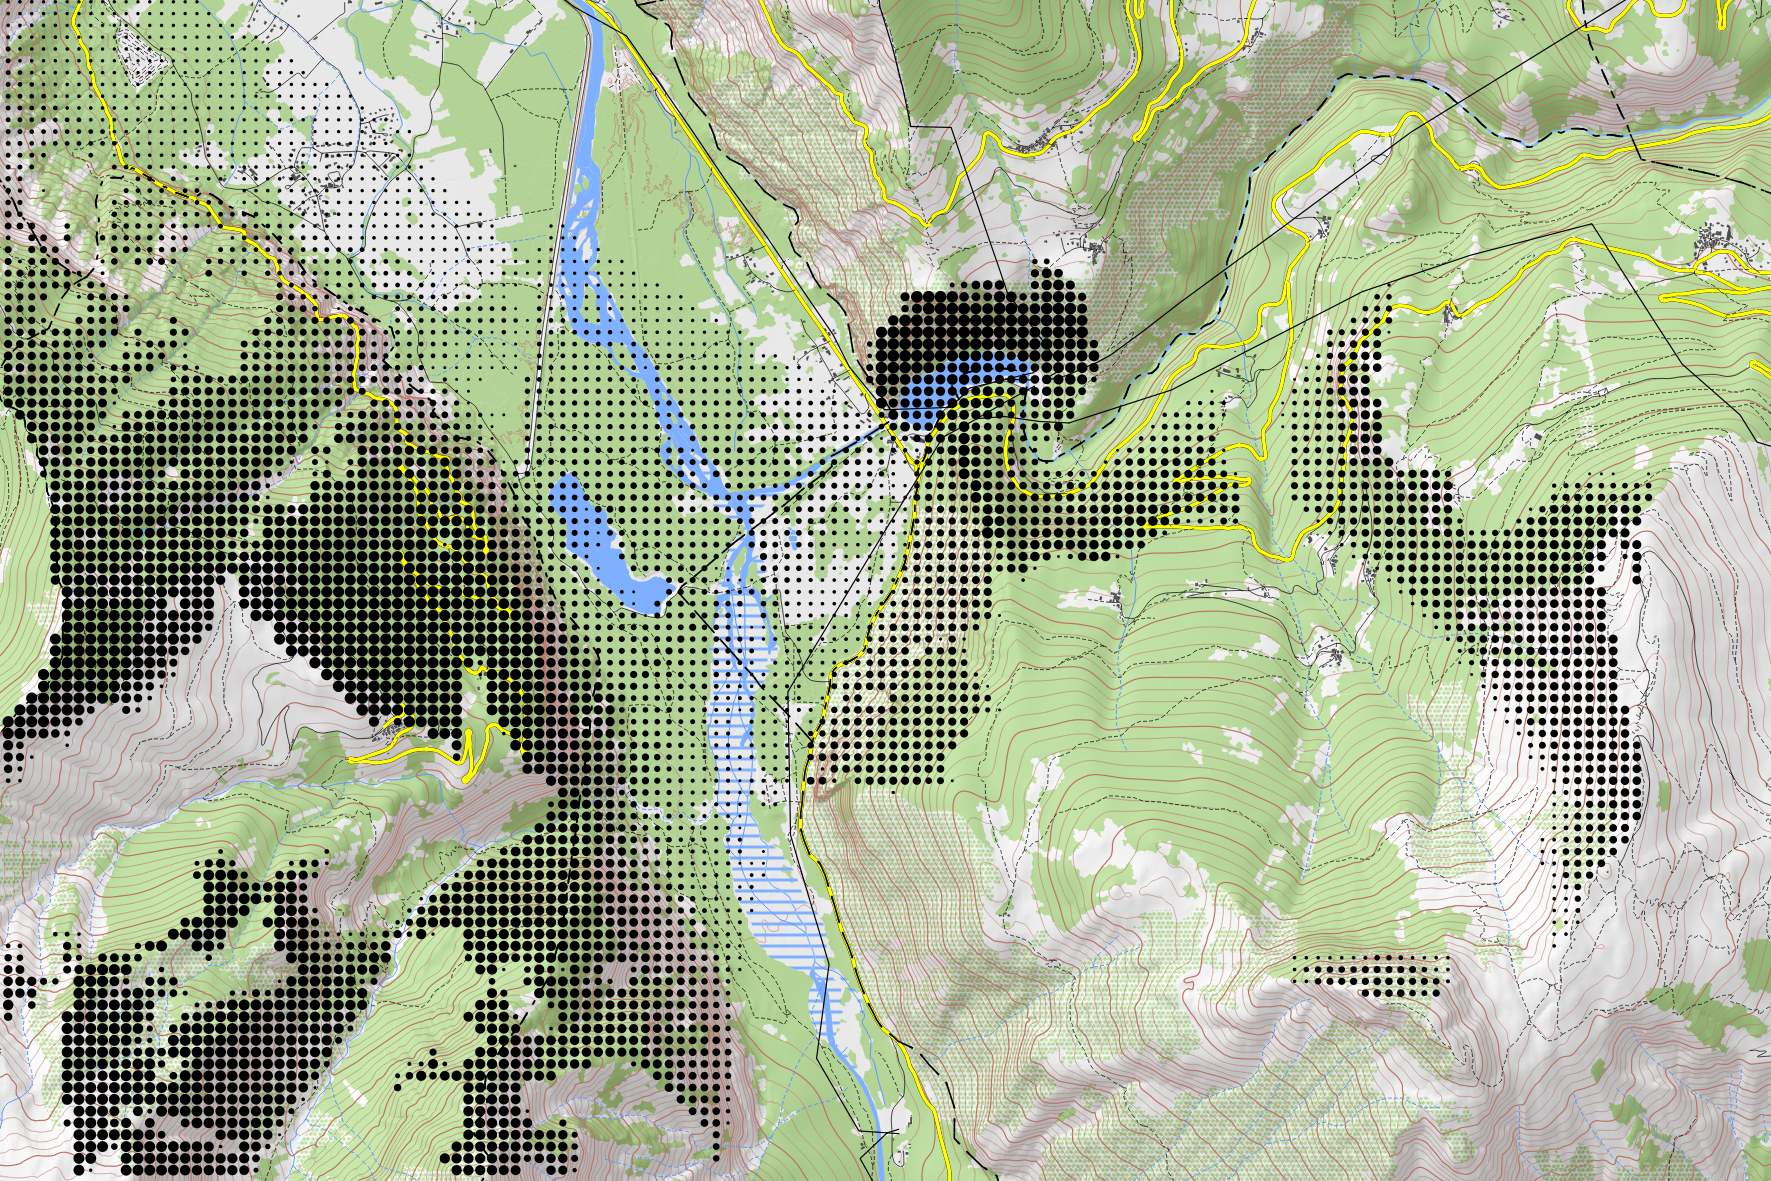
\includegraphics{./figures/Metrique_part_lac_visible.png}};
  %
  \begin{scope}
    \node (P2) at ([yshift=-.5cm]image.south east) {};
    \node (P1) at ([yshift=-.5cm]image.south west) {};
    %
    \foreach \x [evaluate=\xshift using \x/10, evaluate=\rad using (\x * .0004) + .01] in {0,...,100}
    {
      \draw[fill=black,draw=none, below] ([xshift=\xshift cm, yshift=-.5cm]P1) circle [radius=\rad cm];
    }
    %
    \path(P1 |- 0cm,-1cm) --++ (10,0)
    node[et,pos=0] {0}
    node[et,pos=.1] {0,1}
    node[et,pos=.2] {0,2}
    node[et,pos=.3] {0,3}
    node[et,pos=.4] {0,4}
    node[et,pos=.65] {0,65}
    node[et,pos=1] {1};
    % Échelle
    \draw[-] (P2 |- -1cm,-1cm) --++ (-1,0) node[et,pos=.5] {\SI{500}{\meter}};
    % Légende détaillée
    \path (P1) -- (P2) node[pos=.5, yshift=-1cm] {\tiny Pour la légende détaillée du fond topographique voir \autoref{anx:topo_leg}. Sources: BD TOPO 2018, BD ALTI 2018.}; 
  \end{scope}
\end{tikzpicture}
  \caption{Exemple d'une \emph{métrique} issue de la
    \emph{spatialisation} du \emph{fil rouge :} la part de la surface
    visible d'un lac donné.}
  \label{fig:metrique_part_lac}
\end{figure}


\begin{figure}
  \centering
  \begin{tikzpicture}
  \tikzset{et/.style={above,font=\footnotesize\vphantom{Ag}}}
  %
  \node[inner sep=0pt, anchor=south west] (image) at (0,0){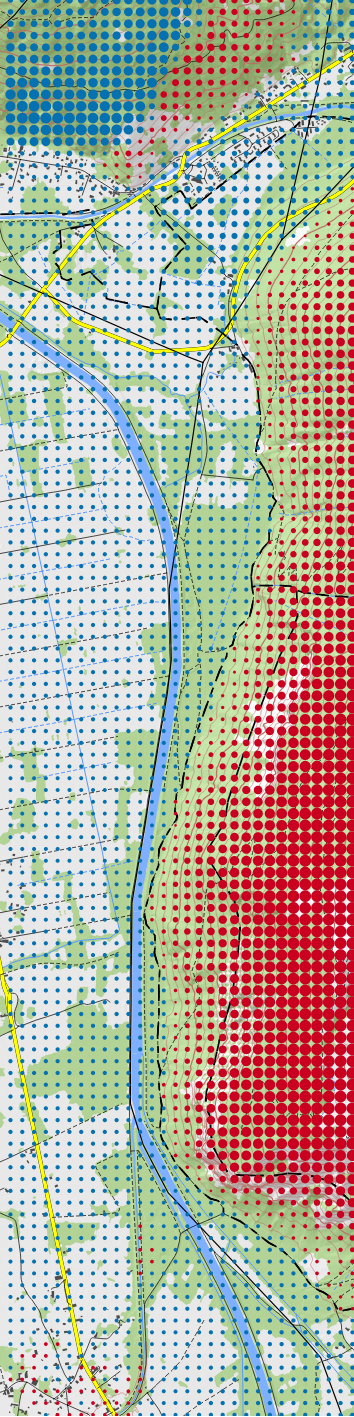
\includegraphics[angle=90]{./figures/Metrique_delta_alt.png}};
  %
  \begin{scope}
    \node (P2) at ([yshift=-.5cm]image.south east) {};
    \node (P1) at ([yshift=-.5cm]image.south west) {};
    %
    \foreach \x [evaluate=\xshift using \x/10, evaluate=\rad using (\x * .0004) + .01] in {0,...,100}
    {
      \draw[fill=black,draw=none, below] ([xshift=\xshift cm, yshift=-.5cm]P1) circle [radius=\rad cm];
    }
    %
    \path(P1 |- 0cm,-1cm) --++ (10,0)
    node[et,pos=0] {0}
    node[et,pos=.1] {0,1}
    node[et,pos=.2] {0,2}
    node[et,pos=.3] {0,3}
    node[et,pos=.4] {0,4}
    node[et,pos=.65] {0,65}
    node[et,pos=1] {1};
    % Échelle
    \draw[-] (P2 |- -1cm,-1cm) --++ (-1,0) node[et,pos=.5] {\SI{500}{\meter}};
    % Légende détaillée
    \path (P1) -- (P2) node[pos=.5, yshift=-1cm] {\tiny Pour la légende détaillée du fond topographique voir \autoref{anx:topo_leg}. Sources: BD TOPO 2018, BD ALTI 2018.}; 
  \end{scope}
\end{tikzpicture}
  \caption{Métrique 2 À  changer ??}
\end{figure}

%%% Local Variables:
%%% mode: latex
%%% TeX-master: "../../../../main"
%%% End:
